\section{Pitch}
\begin{definition}[Pitch]
    Pitch is the property of the sound which allows a relative ordering of perceived sounds on a frequency-related scale.
\end{definition}
On a keyboard, pitch goes up to the right of the keyboard, while it goes down on the left.

Pitches are expressed through \textbf{notes}. There are 7 note names\footnote{C-B in anglophone countries, C-H in Germany and Do-Si for the rest of Europe.}, which are repeated in \textbf{octave registers}, identified by the bottom number.
$$\cdots A_3 B_3 \underbrace{C_4 D_4 E_4 F_4 G_4 A_4 B_4}_{\text{Octave register 4}} C_5 D_5 \cdots$$

\begin{figure}[h]
    \begin{center}
        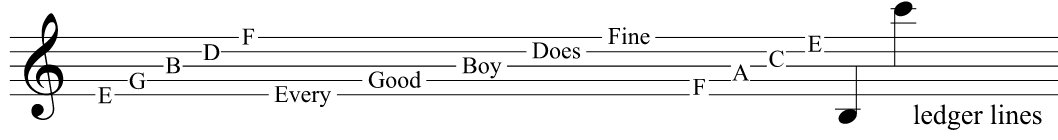
\includegraphics[width=0.8\textwidth]{img/treble}
        \caption{Treble clef}
        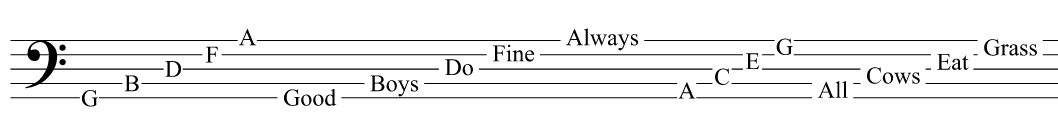
\includegraphics[width=0.8\textwidth]{img/bass}
        \caption{Bass clef}
    \end{center}
\end{figure}

\begin{definition}[Octave]
    The distance / interval between two notes with the same name.
\end{definition}

\begin{definition}[Middle C]
    The $C_4$ pitch, usually located in the middle of a keyboard (on the instrument) and always annotated in the middle of the grand staff, shared by the two staves.
\end{definition}

\begin{figure}[t]
    \begin{center}
        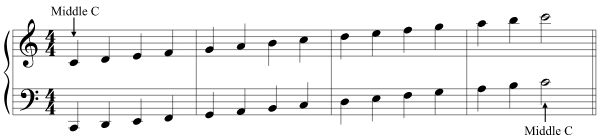
\includegraphics[width=0.8\textwidth]{img/grandstaff}
        \caption{The Grand Staff (a specific stave \emph{system})}
    \end{center}
\end{figure}

\begin{definition}[Accidental]
    A symbol placed before a note to raise / lower its pitch by a given amount.
\end{definition}

An accidental is effective only for a measure. They affect the entire piece if they are placed before the clef in a \textbf{key signature}.
\begin{center}
    \begin{tabular}{r|c|l}
        $\flat{}$ & Flat & $-1$ half step \\
        $\sharp{}$ & Sharp & $+1$ half step \\
        $\musDoubleFlat$ & Double flat & $-2$ half steps / $-1$ whole step \\
        $\musDoubleSharp$ & Double sharp & $+2$ half steps / $+1$ whole step \\
        $\natural{}$ & Natural & Cancels preceding accidentals \\
    \end{tabular}
\end{center}
There exists also \textbf{half-accidentals}, whose altered notes cannot be played on a keyboard.

\begin{definition}[Half step]
    On the keyboard, the distance / interval between one key (either black or white) and the next (either black or white).
\end{definition}

\begin{definition}[Whole step]
    The interval made up of two half steps.
\end{definition}

\begin{figure}[h]
    \begin{center}
        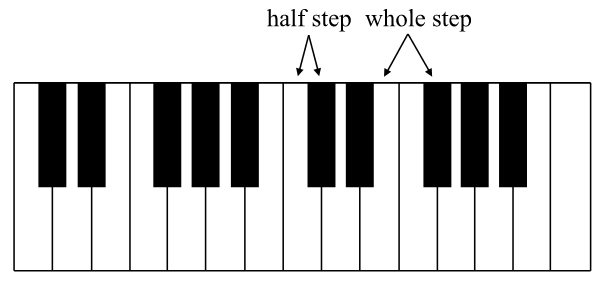
\includegraphics[width=0.6\textwidth]{img/halfstep}
        \caption{Half steps and whole steps}
    \end{center}
\end{figure}

\begin{definition}[Enharmonic]
    Which has the same sound, but different name.
\end{definition}

\section{Rhythm}
\begin{definition}[Beat / pulse]
    The basic pulse underlying measured music and thus the unit by which musical time is reckoned.
\end{definition}

\begin{definition}[Tempo]
    Speed of the beat.
\end{definition}
The tempo is usually expressed through metronome markings in \textbf{BPM / Beats Per Minute}.

\subsection{Time signatures}

\begin{figure}[h]
    \begin{center}
        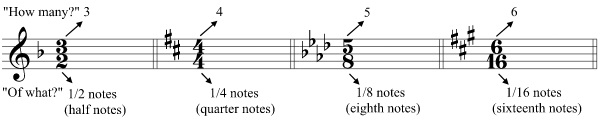
\includegraphics[width=1\textwidth]{img/timesignature}
        \caption{Meaning of the time signatures}
    \end{center}
\end{figure}

\subsection{Note / rests durations}
Both notes and rests last for certain duration, which is always a $2^n$ number of beats, where $n \in \mathbb Z$. Common values for $2^n$ are the following ones:

$$\left\{4,2,1,\frac{1}{2}, \frac{1}{4}\right\} \text{ beats}$$

Values different from these ones can be gathered through \textbf{ties} and \textbf{dots}. A dot adds $\frac{1}{2}$ the value of the note dotted, while a double dot adds $\frac{1}{2} + \frac{1}{4}$ the original value.

\subsection{Meters}
\begin{definition}[Meter]
    Describes the number of beats in a measure / bar and how they are divided.
\end{definition}

\textbf{Simple meters} break the beat into 2 parts, while \textbf{compound meters} break it into 3 parts.

They can be \textbf{double} (2 beats / bar), \textbf{triple} (3 beats / bar) or \textbf{quadruple} (4 beats / bar).

\begin{figure}[h]
    \begin{center}
        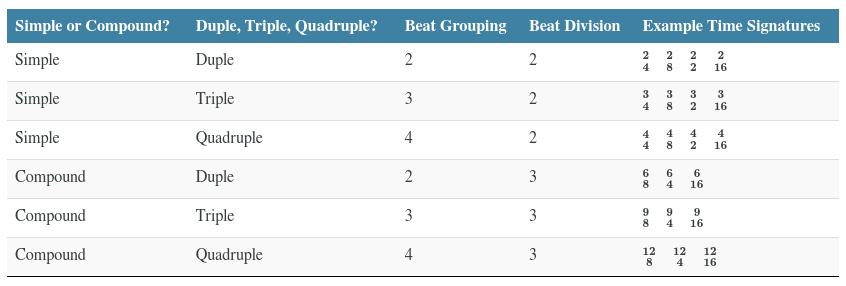
\includegraphics[width=1\textwidth]{img/meters}
        \caption{Meters}
    \end{center}
\end{figure}

\subsection{Tuplets}
\begin{definition}[Tuplet]
    Rhythmic grouping of notes which would typically not occur in the specified meter.
\end{definition}

\begin{definition}[Duplet / Triplet / Quadruplet / Quintuplet]
    Common tuplet instances.
\end{definition}

\subsection{Syncopation}